\documentclass[a4paper,10pt]{article}
\usepackage[utf8]{inputenc}
\usepackage{cite}
\usepackage[top=2.5cm,bottom=2.5cm,left=2.5cm,right=2.5cm]{geometry}
\usepackage[portuguese]{babel}
\usepackage{natbib}
\usepackage{graphicx}
\usepackage{url}



\title{Comércio Eletrônico}
\author{Mader Gabriel de Souza Barbosa}
\date{April, 2022}

\begin{document}

\maketitle

\begin{figure}[h!]
\centering
    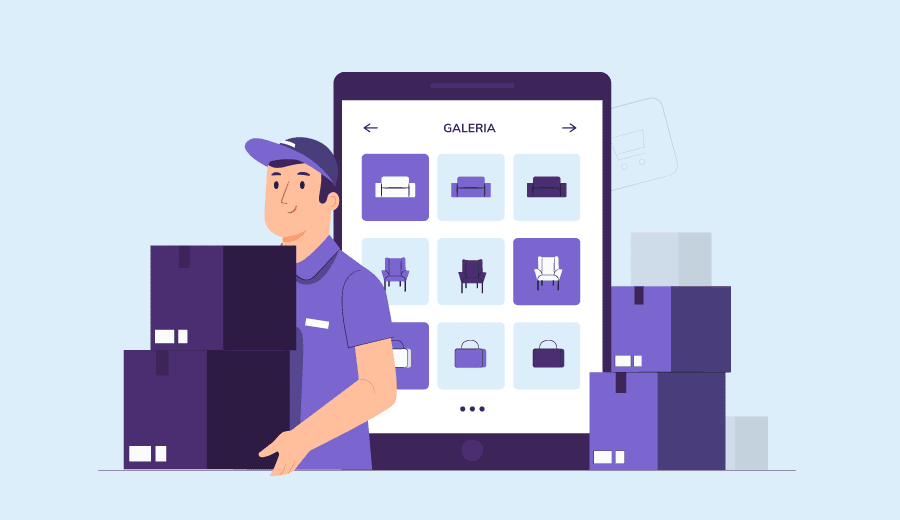
\includegraphics[width=90mm]{ecommerce.png}
    \caption{Ilustração sobre \textit{E-commmerce}. \cite{img:graph}}
    \label{fig:graph1}
\end{figure}

\section{Introdução}
\paragraph 
O comércio eletrônico(ou /textit{E-commerce}) se refere a todas as transações online, sendo inclusa uma ampla gama de atividades online e ferramentas. Se tornando uma das principais alternativas para aumento de ganhos em negócios\cite{img:graph}. Tendo em vista seu grande impacto global, existe uma cadeira eletiva no Centro de Informática(UFPE)  que possui 75 horas de carga horária e visa o estudo e ensino do comércio eletrônico e suas nuances, que é a cadeira IF792.


\section{Relevância}
\paragraph
O valor do comércio eletrônico é dado quando se reflete na possibilidade de mudança que ele proporciona. O \textit{E-commmerce} oferece novas possibilidades para negócios que anteriormente seriam impensáveis, como um pequeno comerciante que devido a esse novo paradigma, pode atender um número muito mais alto de consumidores e de diferentes localizações, muitas vezes lugares distantes. Ademais, essa modalidade de comércio também traz mudanças para outras áreas do comércio que não necessariamente a compra de um produto, mas para com o pós compra(as avaliações, o atendimento ao cliente) e o pré compra(marketing).
\cite{de2016commerce}
\cite{diniz1999comercio}


\section{Relações com outras disciplinas}
\paragraph
Apesar de não necessitar de pré requisito para que a matricula seja feita, a disciplina de comércio eletrônico(IF792), por ser uma disciplina eletiva, irá utilizar alguns conceitos de computação que uma pessoa que não tem conhecimento prévio de matérias dadas nos primeiros períodos do Cin, provavelmente não conseguirá prosperar nesta cadeira, mesmo que não estejam listados de forma obrigatória. Além disso, por ser uma cadeira que é voltada para a área de negócios e empreendedorismo, ela possui relações com outras cadeiras eletivas como gestão de negócios(IF783), negócios online (IF782) e economia para empreendedor (IF780) por serem ligadas à negócios.



\bibliographystyle{plain}
\bibliography{mgsb.bib}

\end{document}
